% Copyright © 2012 Martin Ueding <dev@martin-ueding.de>
%
% Copyright © 2012 Martin Ueding <dev@martin-ueding.de>
%
\documentclass[11pt, ngerman, fleqn]{scrartcl}

\usepackage{graphicx}

%%%%%%%%%%%%%%%%%%%%%%%%%%%%%%%%%%%%%%%%%%%%%%%%%%%%%%%%%%%%%%%%%%%%%%%%%%%%%%%
%                                Locale, date                                 %
%%%%%%%%%%%%%%%%%%%%%%%%%%%%%%%%%%%%%%%%%%%%%%%%%%%%%%%%%%%%%%%%%%%%%%%%%%%%%%%

\usepackage{babel}
\usepackage[iso]{isodate}

%%%%%%%%%%%%%%%%%%%%%%%%%%%%%%%%%%%%%%%%%%%%%%%%%%%%%%%%%%%%%%%%%%%%%%%%%%%%%%%
%                          Margins and other spacing                          %
%%%%%%%%%%%%%%%%%%%%%%%%%%%%%%%%%%%%%%%%%%%%%%%%%%%%%%%%%%%%%%%%%%%%%%%%%%%%%%%

\usepackage[activate]{pdfcprot}
\usepackage[left=3cm, right=2cm, top=2cm, bottom=2cm]{geometry}
\usepackage[parfill]{parskip}
\usepackage{setspace}

\setlength{\columnsep}{2cm}

%%%%%%%%%%%%%%%%%%%%%%%%%%%%%%%%%%%%%%%%%%%%%%%%%%%%%%%%%%%%%%%%%%%%%%%%%%%%%%%
%                                    Color                                    %
%%%%%%%%%%%%%%%%%%%%%%%%%%%%%%%%%%%%%%%%%%%%%%%%%%%%%%%%%%%%%%%%%%%%%%%%%%%%%%%

\usepackage{color}

\definecolor{darkblue}{rgb}{0,0,.5}
\definecolor{darkgreen}{rgb}{0,.5,0}
\definecolor{darkred}{rgb}{.7,0,0}

%%%%%%%%%%%%%%%%%%%%%%%%%%%%%%%%%%%%%%%%%%%%%%%%%%%%%%%%%%%%%%%%%%%%%%%%%%%%%%%
%                         Font and font like settings                         %
%%%%%%%%%%%%%%%%%%%%%%%%%%%%%%%%%%%%%%%%%%%%%%%%%%%%%%%%%%%%%%%%%%%%%%%%%%%%%%%

\usepackage[charter, greekuppercase=italicized]{mathdesign}
\usepackage{beramono}
\usepackage{berasans}

% Style of vectors and tensors.
\newcommand{\tens}[1]{\boldsymbol{\mathsf{#1}}}
\renewcommand{\vec}[1]{\boldsymbol{#1}}

%%%%%%%%%%%%%%%%%%%%%%%%%%%%%%%%%%%%%%%%%%%%%%%%%%%%%%%%%%%%%%%%%%%%%%%%%%%%%%%
%                               Input encoding                                %
%%%%%%%%%%%%%%%%%%%%%%%%%%%%%%%%%%%%%%%%%%%%%%%%%%%%%%%%%%%%%%%%%%%%%%%%%%%%%%%

\usepackage[T1]{fontenc}
\usepackage[utf8]{inputenc}

%%%%%%%%%%%%%%%%%%%%%%%%%%%%%%%%%%%%%%%%%%%%%%%%%%%%%%%%%%%%%%%%%%%%%%%%%%%%%%%
%                         Hyperrefs and PDF metadata                          %
%%%%%%%%%%%%%%%%%%%%%%%%%%%%%%%%%%%%%%%%%%%%%%%%%%%%%%%%%%%%%%%%%%%%%%%%%%%%%%%

\usepackage{hyperref}
\usepackage{lastpage}

\hypersetup{
	breaklinks=false,
	citecolor=darkgreen,
	colorlinks=true,
	linkcolor=black,
	menucolor=black,
	pdfauthor={Martin Ueding},
	urlcolor=darkblue,
}

%%%%%%%%%%%%%%%%%%%%%%%%%%%%%%%%%%%%%%%%%%%%%%%%%%%%%%%%%%%%%%%%%%%%%%%%%%%%%%%
%                               Math Operators                                %
%%%%%%%%%%%%%%%%%%%%%%%%%%%%%%%%%%%%%%%%%%%%%%%%%%%%%%%%%%%%%%%%%%%%%%%%%%%%%%%

\usepackage[thinspace, squaren]{SIunits}
\usepackage{amsmath}
\usepackage{amsthm}
\usepackage{commath}

% Word like operators.
\DeclareMathOperator{\arcsinh}{arsinh}
\DeclareMathOperator{\arsinh}{arsinh}
\DeclareMathOperator{\asinh}{arsinh}
\DeclareMathOperator{\card}{card}
\DeclareMathOperator{\diam}{diam}
\renewcommand{\Im}{\mathop{{}\mathrm{Im}}\nolimits}
\renewcommand{\Re}{\mathop{{}\mathrm{Re}}\nolimits}

% Special single letters.
\DeclareMathOperator{\fourier}{\mathcal{F}}
\newcommand{\C}{\ensuremath{\mathbb C}}
\newcommand{\ee}{\mathrm e}
\newcommand{\ii}{\mathrm i}
\newcommand{\N}{\ensuremath{\mathbb N}}
\newcommand{\R}{\ensuremath{\mathbb R}}

% Shape like operators.
\DeclareMathOperator{\dalambert}{\Box}
\DeclareMathOperator{\laplace}{\bigtriangleup}
\newcommand{\curl}{\vnabla \times}
\newcommand{\divergence}[1]{\inner{\vnabla}{#1}}
\newcommand{\vnabla}{\vec \nabla}

% Shortcuts
\newcommand{\ev}{\hat{\vec e}}
\newcommand{\e}[1]{\cdot 10^{#1}}
\newcommand{\half}{\frac 12}
\newcommand{\inner}[2]{\left\langle #1, #2 \right\rangle}

% Placeholders.
\newcommand{\emesswert}{\del{\messwert \pm \messwert}}
\newcommand{\fehlt}{\textcolor{darkred}{Hier fehlen noch Inhalte.}}
\newcommand{\messwert}{\textcolor{blue}{\square}}
\newcommand{\punkte}{\textcolor{white}{xxxxx}}


\usepackage{fancyhdr}
\usepackage{tikz}

\usetikzlibrary{arrows}
\usetikzlibrary{intersections}


\newcommand{\themodul}{physik311}
\newcommand{\thegruppe}{Gruppe 3 -- Matthias Rehberger}
\newcommand{\theuebung}{8}

\pagestyle{fancy}

\fancyfoot[C]{\footnotesize{\thegruppe}}
\fancyfoot[L]{\footnotesize{Martin Ueding}}
\fancyfoot[R]{\footnotesize{Seite \thepage\ / \pageref{LastPage}}}
\fancyhead[L]{\themodul{} -- Übung \theuebung}

\setcounter{section}{26}

\def\thesubsection{\thesection\alph{subsection}}

\title{\themodul{} -- Übung \theuebung \\ \vspace{0.5cm} \large{\thegruppe}}

\author{Martin Ueding \\ \small{\href{mailto:mu@uni-bonn.de}{mu@uni-bonn.de}}}

\begin{document}

\maketitle

\begin{table}[h]
	\centering
	\begin{tabular}{l|c|c|c|c}
		Aufgabe & \ref{1} & \ref{2} & \ref{3} & $\sum$   \\
		\hline
		Punkte & \punkte & \punkte & \punkte & \punkte
	\end{tabular}
\end{table}

%%%%%%%%%%%%%%%%%%%%%%%%%%%%%%%%%%%%%%%%%%%%%%%%%%%%%%%%%%%%%%%%%%%%%%%%%%%%%%%
%                                 Newtonringe                                 %
%%%%%%%%%%%%%%%%%%%%%%%%%%%%%%%%%%%%%%%%%%%%%%%%%%%%%%%%%%%%%%%%%%%%%%%%%%%%%%%

\section{Newtonringe}
\label 1

\subsection{Herleitung der Formel}

Falls in dieser Aufgabe auch die Herleitung der Formel gefragt war:
\cite{wikipedia-newtonringe}

\begin{figure}
	\centering
	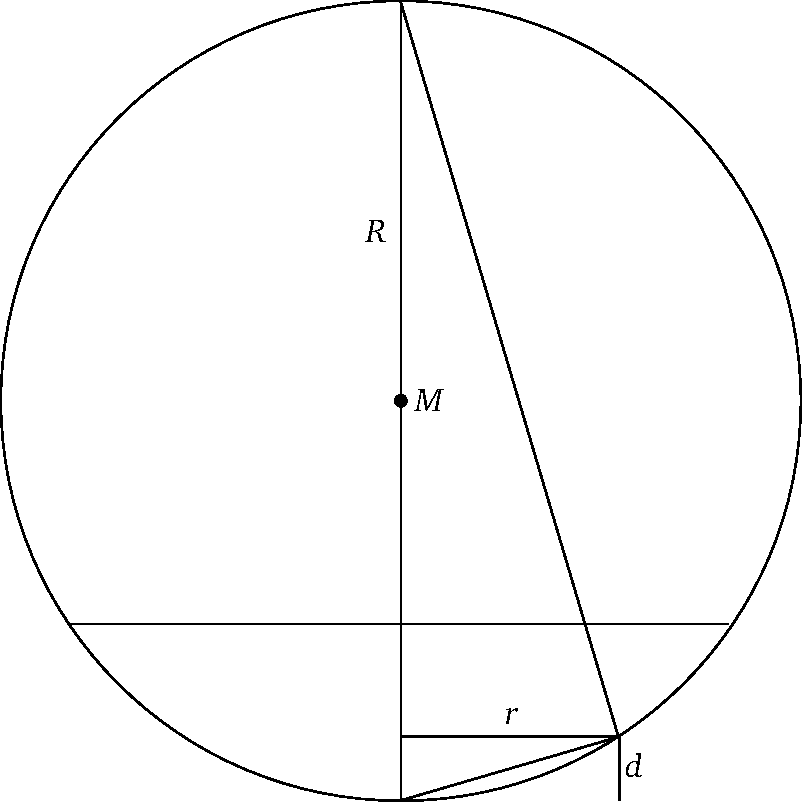
\includegraphics[width=0.5\textwidth]{27-Skizze.pdf}
	\caption{Skizze zur Herleitung der Newtonringe}
	\label{fig:newton}
\end{figure}

Die brechende Wirkung der Linse kann ich vernachlässigen, da der
Krümmungsradius sehr groß ist. In Abbildung \ref{fig:newton} habe ich einige
Strecken benannt. Da das Licht nahezu senkrecht einfällt, ist die Strecke, die
das Licht in der Luft nach der Linse zurücklegt, $2 d$. Strahlen, die innen
in der Linse reflektiert werden, legen keinen Weg in Luft zurück. Die Reflexion
an der Glasplatte ist allerdings am optisch dichteren Medium, somit kommt noch
eine Phasenverschiebung um $\pi$ dazu. Das entspricht einem Mehrweg von
$\lambda/2$.  Die Reflexion innen in der Linse erzeugt keine
Phasenverschiebung.

Der Gangunterschied (also der Mehrweg des ersten Strahls) muss gerade ein
ungerades Vielfache der halben Wellenlänge sein, damit es zur Auslöschung
kommt:
\[
	2d + \frac \lambda 2 = \del{n + \half} \lambda
	\iff
	2d = n \lambda
\]

Nun soll noch $d$ durch $r$ ausgedrückt werden. Dazu benutze ich den Höhensatz.
Das rechtwinklige Dreieck ist das Große, dass den rechten Winkel auf dem Kreis
hat (Satz des Thales). Dann gilt:
\[
	d (2R - d) = r^2
\]

Aufgrund des großen Krümmungsradius kann dies genähert werden zu:
\[
	2dR = r^2
\]

Dies setze ich ein und stelle nach $r$ um. Ich erhalte:
\[
	r = \sqrt{\lambda n R}
\]

\subsection{Einsetzen der Werte}

Ich setze in die Formel $r = \sqrt{\lambda n R}$ ein und erhalte den Radius des
$n$-ten Ringes:
\[
	r = \sqrt{n} \cdot \unit{2.19317}{\milli\meter}
\]

Nun setze ich $r = \unit{2}{\centi\meter}$ ein und löse nach $n$ auf. Ich
erhalte $n = 83.16$. Es gibt also $83$ Ringe.

%%%%%%%%%%%%%%%%%%%%%%%%%%%%%%%%%%%%%%%%%%%%%%%%%%%%%%%%%%%%%%%%%%%%%%%%%%%%%%%
%                            Fabry-Perot Resonator                            %
%%%%%%%%%%%%%%%%%%%%%%%%%%%%%%%%%%%%%%%%%%%%%%%%%%%%%%%%%%%%%%%%%%%%%%%%%%%%%%%

\section{Fabry-Perot Resonator}
\label 2

\subsection{Abstand und Reflektivitäten}

Den Abstand $d$ kann ich über den freien Spektralbereich bestimmen, dabei ist
$n = 1$:
\[
	\Deltaup f = \frac{c}{2dn}
	\implies
	d = \unit{74.9481}{\centi\meter}
\]

Die Reflektivität $R$ kann ich über die Finesse $\mathcal F$ bestimmen:
\[
	\mathcal F = \frac{\pi \sqrt{R}}{1-R}
	\implies
	R = 0.989583
\]


\subsection{Leistungsüberhöhung}

Bei einer Finesse von $300$ sollte die Leistung im Resonator
$\unit{300}{\watt}$ sein.

\subsection{Speicherzeit}

Pro Reflexion verliert der Resonator einen Anteil von $1/300$ seiner Strahlen.
Somit gilt für die Stahlenanzahl im Resonator:
\[
	\dot n = - \frac{1}{300} n
\]

Dies wird gelöst durch:
\[
	n(k) = n(0) \ee^{-k/300}
\]

Der Wert $1/\ee$ ist genau dann erreicht, wenn $k = 300$, also nach $300$
Reflexionen.

Mit der Lichtgeschwindigkeit $c$ und dem Spiegelabstand $d$ entspricht dies
einer Zeit von:
\[
	t = \frac{k d}{c} = \frac{k}{2n \Deltaup f}
	\implies
	t = \unit{75}{\nano\second}
\]

Dies ist auch gleich der Zusammenhang zwischen $t$ und $\Deltaup f$.

%%%%%%%%%%%%%%%%%%%%%%%%%%%%%%%%%%%%%%%%%%%%%%%%%%%%%%%%%%%%%%%%%%%%%%%%%%%%%%%
%                         das Michelsoninterferometer                         %
%%%%%%%%%%%%%%%%%%%%%%%%%%%%%%%%%%%%%%%%%%%%%%%%%%%%%%%%%%%%%%%%%%%%%%%%%%%%%%%

\section{das Michelsoninterferometer}
\label 3

\subsection{Intensitäten}

Ich gehe davon aus, dass die Dicke des Strahlteilers zu vernachlässigen ist.
Der Gangunterschied alleine wird eine Phasenverschiebung $\delta$ des zweiten
Strahls gegenüber dem ersten hervorrufen. Dabei ist $k = \omega/c$ die
Wellenzahl in $\radian\per\meter$.
\[
	\delta = k \underbrace{(s_2 - s_1)}_g
\]

Der erste Strahl wird vom Strahlteiler nicht verschoben. Beim Detektor wir dieser Strahl ohne weitere Phasenverschiebung durch den Strahlteiler ankommen, der zweite Strahl wird jedoch am optisch dichteren Medium reflektiert und bekommt somit eine Verschiebung von $\pi$ dazu. Die relative Phase zwischen den beiden Strahlen ist dann um $\pi$ großer.

Beim Laser kommt es anders an, dort wurde der erste Strahl wieder am optisch
dünneren Medium reflektiert und somit nicht phasenverschoben. Der zweite Strahl
wird jedoch gar nicht am Strahlteiler reflektiert, somit entfällt die
Phasenverschiebung. 

Die Amplituden $\vec A_i$ der beiden Strahlen addieren sich vektoriell, wie in Abbildung \ref{fig:3} dargestellt. Die Intensität ist die Summe der Amplituden zum Quadrat. Somit gilt:
\[
	\vec A = \vec A_1 + \vec A_2 = A_0 \del{ \begin{pmatrix}
	1 \\ 0
	\end{pmatrix} + \begin{pmatrix}
		\cos\del\delta \\ \sin\del\delta
	\end{pmatrix} }
\]

\begin{figure}
	\centering
	\begin{tikzpicture}
		\draw[->] (0, 0) -- ++(0:2) node[midway, below] {$\vec A_1$};
		\draw[->] (0:2) -- ++(30:2) node[midway, below] {$\vec A_2$};
	\end{tikzpicture}
	\caption{Zeigerdiagram für die Phasenverschiebung}
	\label{fig:3}
\end{figure}

Das Quadrat ist:
\[
	I = A_0^2 \del{\del{1 + \cos\del\delta}^2 + \sin^2\del\delta}
	= 2 A_0^2 \del{1 + \cos\del\delta}
\]

Die Intensität kann sich also verdoppelt oder auslöschen.

Beim Detektor wird also folgende Intensitätsverteilung ankommen. Dabei habe ich
$\cos(x + \pi) = - \cos(x)$ benutzt:
\[
	I(g) = 2 A_0^2 \del{1 - \cos\del{kg}}
\]

Beim Spiegel:
\[
	I(g) = 2 A_0^2 \del{1 + \cos\del{kg}}
\]

\subsection{Verkippung}

Ich verkippe den \emph{Spiegel 1}, den \emph{Spiegel 2} lasse ich stehen. Der
Verkippungswinkel $\psi$ des Wellenvektors wird durch eine Verkippung des
Spiegels um $\psi/2$ erreicht.

Bisher sind die beiden Wellen in Winkel von $\pi/2$ aufeinander getroffen. Das
heißt, dass entlang der teilreflektierenden Seite, die genau im $\pi/4$ Winkel
zu den beiden Strahlen liegt, beide Strahlen die gleiche Wellenzahl haben und
somit das Interferenzmuster konstant ist.

Ich parametrisiere die teilreflektierende Kante ihrer Länge nach mit der
Koordinate $a$. Für die noch nicht verkippten Strahlen gilt dann für deren
Phase $\phi$ mit Wellenzahl $k$:
\[
	\phi_1(a) = \phi_1(0) + \sin\del{\frac \pi 4} ak
	,\quad
	\phi_2(a) = \phi_2(0) + \cos\del{\frac \pi 4} ak
\]

Interessant ist die Phasendifferenz der beiden Wellen:
\[
	\Deltaup \phi(a)
	= \phi_2(0) - \phi_1(0) + \del{\cos\del{\frac \pi 4} - \sin\del{\frac \pi 4}} ak
	= \Deltaup \phi(0)
\]

Wie schon vorher überlegt, hängt die Phasendifferenz (und damit die Intensität der erzeugten Welle) nicht vom Ort $a$ ab. Mit der Verkippung um $\psi$ gilt jetzt:
\[
	\phi_1(a) = \phi_1(0) + \sin\del{\frac \pi 4 + \psi} ak
	,\quad
	\phi_2(a) = \phi_2(0) + \cos\del{\frac \pi 4} ak
\]

Jetzt ist die Differenz nicht mehr konstant:
\begin{align*}
	\Deltaup \phi(a)
	&= \phi_2(0) - \phi_1(0) + \del{\cos\del{\frac \pi 4} - \sin\del{\frac \pi 4 + \psi}} ak \\
	&= \Deltaup \phi(0) + \del{\cos\del{\frac \pi 4} - \sin\del{\frac \pi 4}\cos\del\psi - \cos\del{\frac \pi 4}\sin\del\psi} ak \\
	\intertext{%
		Praktischerweise sind $\cos\del{\pi/4}$ und $\sin\del{\pi/ 4}$ gleich,
		so dass ich beides ausklammern kann.
	}
	&= \Deltaup \phi(0) + \cos\del{\frac \pi 4} \del{1 - \cos\del\psi - \sin\del\psi} ak
\end{align*}

Nun addiere ich wieder die beiden Wellen mit Phase $0$ und $\Deltaup \phi(a)$ um die Amplitude der resultierende Welle zu erhalten. Dabei benutze ich die Formel, die ich vorher schon für die Intensität hatte:
\[
	I(a) = 2 A_0^2 \del{1 + \cos\del{\Deltaup \phi(0) + \cos\del{\frac \pi 4} \del{1 - \cos\del\psi - \sin\del\psi} ak}}
\]

Die Funktion $I(a)$ ist in Abbildung \ref{fig:1} und \ref{fig:2} geplottet.

\begin{figure}
	\centering
	\begin{minipage}[t]{0.43\linewidth}
	\centering
	\includegraphics[width=\linewidth]{28-1.pdf}
	\caption{%
		Interferenzmuster, $I$ gegen $a$. Es ist ein bestimmter
		Verkippungswinkel $\psi$ ist eingestellt, der Gangunterschied $\Deltaup
		\phi(0)$ ist gleich $0$.
	}
	\label{fig:1}
	\end{minipage}
	\hspace{0.12\linewidth}
	\begin{minipage}[t]{0.43\linewidth}
	\centering
	\includegraphics[width=\linewidth]{28-2.pdf}
	\caption{%
		Interferenzmuster, $I$ gegen $a$. Gangunterschied $\Deltaup \phi(0)
		\neq 0$.
	}
	\label{fig:2}
	\end{minipage}
\end{figure}

\bibliography{../../zentrale_BibTeX/Central}
\bibliographystyle{plain}

\end{document}

% vim: spell spelllang=de
